\documentclass[12pt]{article}
\PassOptionsToPackage{quiet}{fontspec}
\usepackage[a4paper, total={6.5in, 10in}]{geometry}
\usepackage{amsmath}
\usepackage{tikz}
\usepackage{ctex}
\usepackage{pgfplots}
\pgfplotsset{compat=1.17}
\usepackage{xcolor}
\usepackage{float}
\usepackage{enumerate}
\usepackage{multicol}

\newcommand{\sep}{\noindent\rule{0.95\linewidth}{2pt}\par}


\title{TikZ使用技巧}
\author{Eureka}
\date{\today}
\begin{document}
\maketitle
\tableofcontents
\clearpage

\section{序言}
在平常使用tikz的过程中一般都是draw和node,根本不考虑什么复杂的东西。
有时候这两玩意儿不行了就使用一个overlay【doge】。
但是技巧这个东西,是你用出来的,你不去用,看一万个也是白瞎 。。。
距离我上一次更新TiKZ相关的东西还是在上次了,该更新一下了。


\section{总述}
本文的主要内容如下:

\begin{multicols}{2}
    \begin{enumerate}[(1)]
        \item node的偏移
        \item node的坐标运算
        \item path的使用
        \item decoration的使用
        \item 高光的使用
        \item overlay详解
        \item 三维图形绘制
        \item 分隔符(Delimiters)
        \item tikz-euclide宏包使用初步
        \item standalone文档类(制作壁纸)
        \item 数学字体配置(mtpro2-lite)
        \item tcolorbox配置入门
        \item 3维统计图
        \item 矩阵元素高亮
    \end{enumerate}
\end{multicols}


\section{overlay}
其实就是在已有内容的位置上再添加一些标记,比如画线,添加标注。
很多人不是说 \LaTeX{} 中的图片排版很废物吗,那么就用tikz的overlay
选项即可。这样你想放在哪里就放在哪里。



\section{node相关}
\subsection{node偏移}
其实就是下面这个语法格式:

\sep
\begin{verbatim}
\draw[->] (0.75, 2) node[below right = 15pt and 2pt]{$\C{F}_1$}--(0.75, 1);
% 错误的写法 node[below=15pt,right=2pt]
% 这样它的效果就是只有right的作用,原来的below作用被覆盖了。
\end{verbatim}
其实这个技巧我觉得挺实用的,你就不用去修改点的坐标了。



\subsection{node坐标运算}
其实就是当你标记了几个node之后,你想要在他们的某些几何中心作图,可以直接调用内置操作
完成,没有必要1pt的调整了。

\clearpage
\section{decoration的使用}
就是一些装饰用的路径,常用的有:花括号,蛇形等。就比如下面这个例子

\sep
\begin{verbatim}
\draw[decorate,decoration={calligraphic brace}](1, 1)--(1, 0)node{SupperMartingle};
\end{verbatim}

\section{三维图形绘制}
基本的坐标轴和部分的预定义平面

\begin{figure}[!htb]
    \centering
    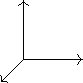
\includegraphics[scale=1]{./pics/coor-3d.pdf}
    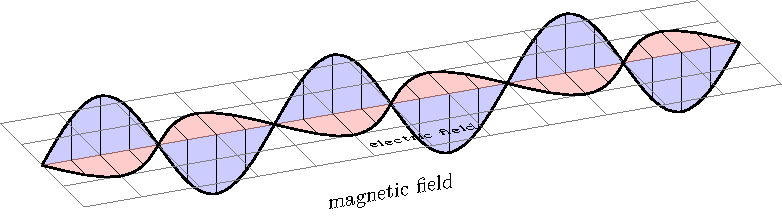
\includegraphics[scale=1]{./pics/dna.pdf}
\end{figure}



\section{高光使用}
在谈到怎么使用高管时,我们首先说明tikz中的{\ttfamily colormap}.
在 tikz 中有着很多的已经定义好的{\ttfamily colormap}:
\begin{itemize}
    \item cool
    \item bluered
\end{itemize}


下面是使用colormap对函数绘制的渐变影响.
\begin{center}
    \centering
    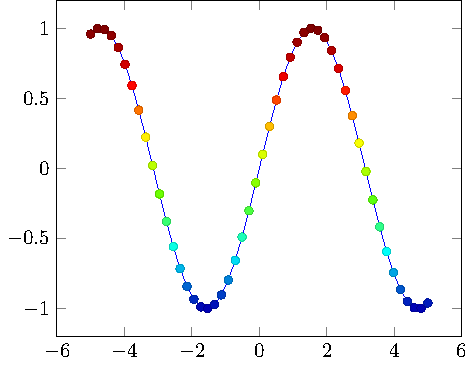
\includegraphics[scale=1]{./pics/fig1-1.pdf}
    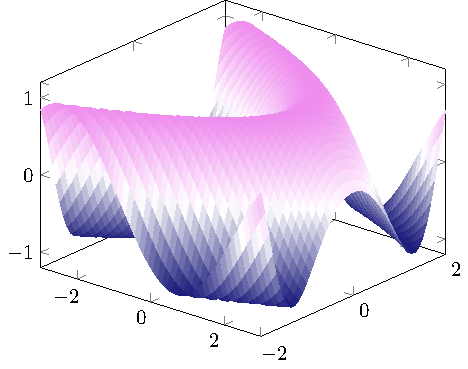
\includegraphics[scale=1]{./pics/fig1-2.pdf}
\end{center}


三维  bar diagram 绘制,我主要例举了如下的两个示例:

\begin{center}
    \centering
    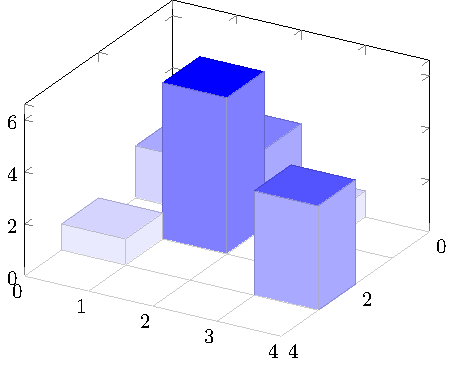
\includegraphics[scale=1]{./pics/fig2-1.pdf}
    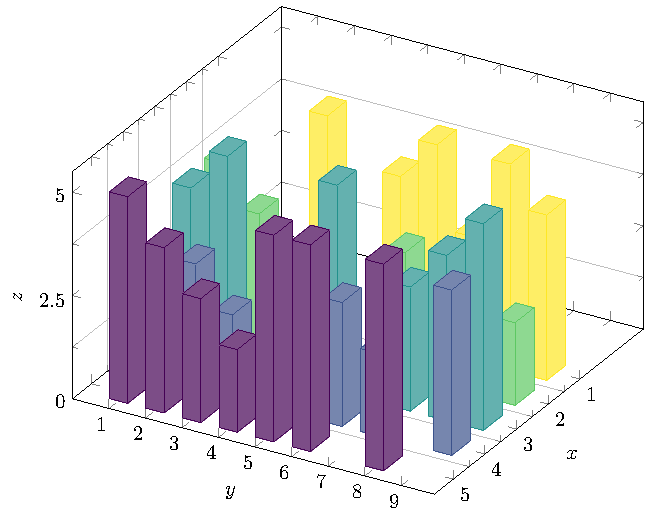
\includegraphics[scale=.7]{./pics/fig2-2.pdf}
\end{center}


\section{数学字体配置}
\section{tikz-euclide宏包初步}
\section{tcolorbox配置}


\section{Delimiters}
主要就是我们该给组公式使用大括号 

\subsection{基础括号}
\begin{figure}[!htb]
    \centering
    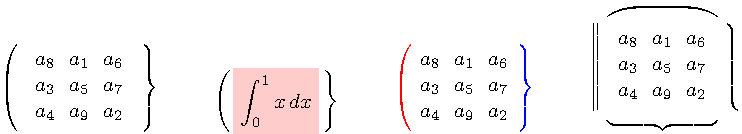
\includegraphics[scale=1]{./pics/brace.pdf}
\end{figure}



\subsection{自定义path 为 Delimiters}
首先的说明什么是 {\ttfamily path, Delimiters},
其实 {\ttfamily Delimiters} 就是分隔符。


\clearpage
\section{Branchs}
\begin{figure}[!htb]
    \centering
    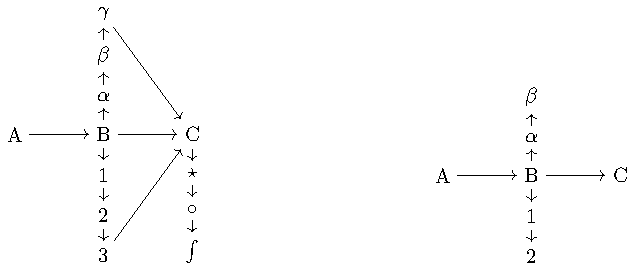
\includegraphics[scale=1]{./pics/branch.pdf}
\end{figure}


\section{流程图}
\begin{figure}[!htb]
    \centering
    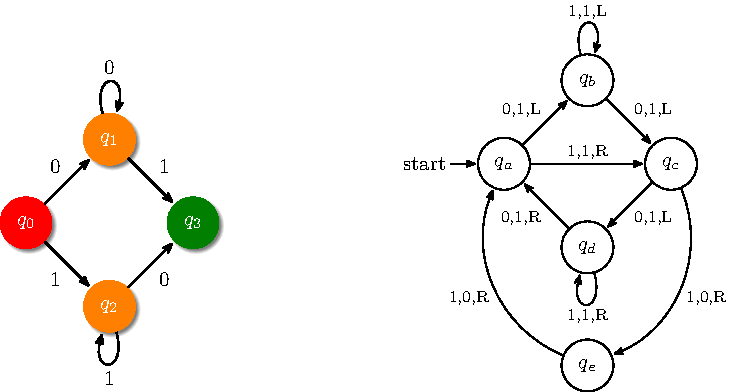
\includegraphics[scale=1]{./pics/process.pdf}
\end{figure}


\end{document}